\chapter{New Framework}

\subsection{Small and Simple Core}

\paragraph{Pipes and Connectors} +figuur

\paragraph{Connections} % niet beginnen over async stuff, later "gebruiken"

\subsection{Some useful pipes}

\paragraph{Merge and Split}

\paragraph{Filter}

\subsection{Extending to fit our needs}

\paragraph{Pipes with memory} 

\paragraph{Flow enrichment}

\paragraph{Parsers}

\paragraph{Asynchronous connections}

\paragraph{Locking}

\section{Practical applications}

\subsection{Dependency Resolution}

\subsection{Concurrent, incremental Clustering}

Clustering is a very important step in building towards a solution. Each new flow of information indirectly leads to a clustering operation. Acquiring new information triggers rules which on their turn yield similarities. These similarities change the balance between clusters. In the worst case, an expensive rebalancing procedure is necessary.

It is obvious that processing similarities is something that will be executed very frequently (numbers?). The combination of the enormous amount of similarities and their expensive processing requires us to make this process as streamlined and efficient as possible. The clustering algorithm as explained in [REF] leads to a first, na\"ive implementation approach. Rethinking the absolute needs of the clustering algorithm then leads to a second approach that benifits greatly of the foundations of our framework.

\paragraph{In-graph implementation} The most simple solution one can think of is to maintain the ICW and OCW for every vertex in the vertex itself. The adjacency matrix would implicitly be defined by the edges between two nodes in the similarity plane. This technique has two main drawbacks:

\begin{enumerate}
\item A lot of load would be pushed to the database.
\item There would be a need for several concurrency control mechanisms/
\end{enumerate}

If clustering could be executed without the use of the database in an efficient manner, it would be preferrable. After all it is in our best interest to take as much load as possible away from the database because it is much more difficult to scale than our pipes and filters architecture. Besides, the similarity ``meta''-plane is not something that should be queried from our end-user application. The users are interested in the result of the clustering, not the way it got there.

In the case of similarities being processed in parallel, we need to pay some extra attention. We do not want that the clustering mechanism inflicts race conditions and, by consequence, inconsistencies on the graph.


\paragraph{As a stateful pipe}

\begin{algorithm}
\caption{!!!}
\label{mincutgusfield}
\begin{algorithmic}
\STATE \textbf{lock} $I_1,I_2$
\IF{cluster($I_1$) == cluster($I_2$)}
  \STATE \textbf{watch} $C_1,C_2$
  \STATE \textbf{unlock} $I_1,I_2$
  \STATE \textbf{process(intra-cluster)}
\ELSE
  \STATE \textbf{lock} $C_1,C_2$
  \STATE \textbf{unlock} $I_1,I_2$
  \STATE \textbf{process(inter-cluster)}
  \STATE \textbf{execute}
  \STATE \textbf{unlock} $C_1,C_2$
\ENDIF
\end{algorithmic}
\end{algorithm}

\begin{figure}[htbp]
	\centering
		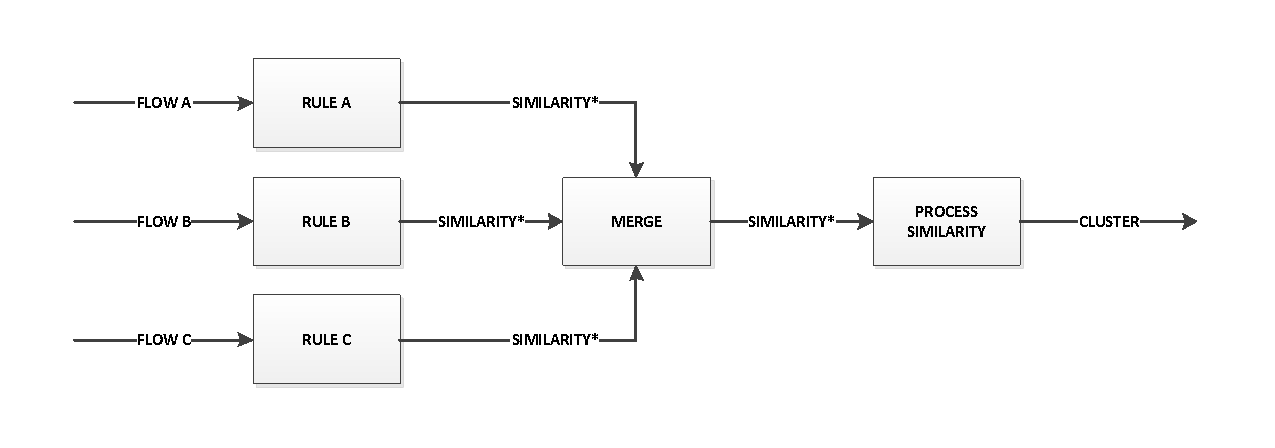
\includegraphics[width=1\textwidth]{fig/clusteringpipe}
	\caption{Clustering flow}
	\label{fig:clusteringpipe}
\end{figure}

\subsection{Assignment of e-mail addresses}